\section{Εισαγωγή}

Στην παρούσα ενότητα εξετάζεται η εφαρμογή της μεθόδου ταυτοποίησης Matrix Pencil (MP) σε αποκρίσεις διαταραχών που προκύπτουν από δυναμικές προσομοιώσεις στο περιβάλλον \textenglish{\textit{PowerFactory}}. Η μεθοδολογία εφαρμόζεται σε χρονοσειρές τάσης ($V$), ρεύματος ($I$), ενεργού ($P$) και άεργου ($Q$) ισχύος, μετά από κατάλληλη προεπεξεργασία, με στόχο την εξαγωγή και τον χαρακτηρισμό των κυρίαρχων ταλαντωτικών ιδιοτιμών και την αξιολόγηση της ποιότητας της ανακατασκευής των σημάτων.

Η διερεύνηση πραγματοποιείται σε δύο Συστήματα Ηλεκτρικής Ενέργειας διαφορετικής κλίμακας και πολυπλοκότητας, στο \textenglish{\textit{Kundur Two-Area System}}~\cite{kundur1994} και στο \textenglish{\textit{IEEE 39-Bus System}}~\cite{digsilent39,pai1989}. Με αυτόν τον τρόπο, η αναφορά δεν περιορίζεται μόνο σε ένα κλασικό δοκιμαστικό σύστημα αναφοράς, αλλά επιτρέπει τη συγκριτική αξιολόγηση της συμπεριφοράς της μεθόδου ως προς την αναγνώριση \textenglish{\textit{inter-area}} και \textenglish{\textit{intra-area}} ρυθμών ταλάντωσης.

\subsection{Εξεταζόμενα συστήματα}

Για τη μελέτη και την επαλήθευση των αλγορίθμων εκτίμησης και συσταδοποίησης ιδιοτιμών, το σύστημα δοκιμής 2 Περιοχών--4 Γεννητριών του Kundur (\textenglish{\textit{Kundur Two-Area 4-Generator Benchmark System}}) αποτελεί διεθνές πρότυπο αναφοράς. Το συγκεκριμένο σύστημα αποτελείται από δύο περιοχές που συνδέονται μέσω μιας διπλής ασθενούς διασυνδετικής γραμμής και εμφανίζει καθαρά διακριτούς τοπικούς τρόπους ταλάντωσης εντός κάθε περιοχής~\cite{kundur1994,klein1991interarea}. Το μονογραμμικό του διάγραμμα παρουσιάζεται στο Σχήμα~\ref{fig:examined-kundur-system}.

\begin{figure}[htbp]
    \centering
    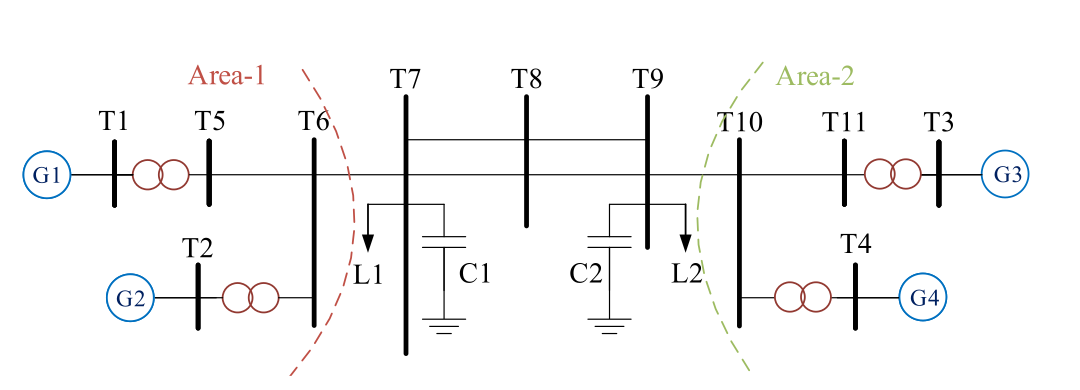
\includegraphics[width=0.92\textwidth]{images/system_figures/kundur_two_area_from_estimation2021.png}
    \caption{Μονογραμμικό διάγραμμα του \textenglish{\textit{Kundur Two-Area System}}. Πηγή:~\cite{estimation2021}.}
    \label{fig:examined-kundur-system}
\end{figure}

Το πρότυπο σύστημα \textenglish{\textit{IEEE 39-Bus}} (\textenglish{\textit{New England Power System}}) αποτελεί ευρέως αποδεκτό σύστημα αναφοράς για μελέτες δυναμικής ευστάθειας και ταλαντώσεων ευρείας περιοχής. Αποτελείται από 39 ζυγούς, 10 γεννήτριες, εκ των οποίων η μία αναπαριστά ισοδύναμο διασύνδεσης μεγάλης έκτασης, 19 φορτία και 46 γραμμές μεταφοράς/μετασχηματιστές. Το σύστημα εμφανίζει τοπικούς και διασυνδετικούς ρυθμούς ταλάντωσης, καθιστώντας το κατάλληλο για την αξιολόγηση και σύγκριση της ακρίβειας των αλγορίθμων συσταδοποίησης υπό διαφορετικά σενάρια διείσδυσης ΑΠΕ και τύπων φορτίου~\cite{digsilent39,estimation2021}. Το μονογραμμικό του διάγραμμα παρουσιάζεται στο Σχήμα~\ref{fig:examined-ieee39-system}.

\begin{figure}[htbp]
    \centering
    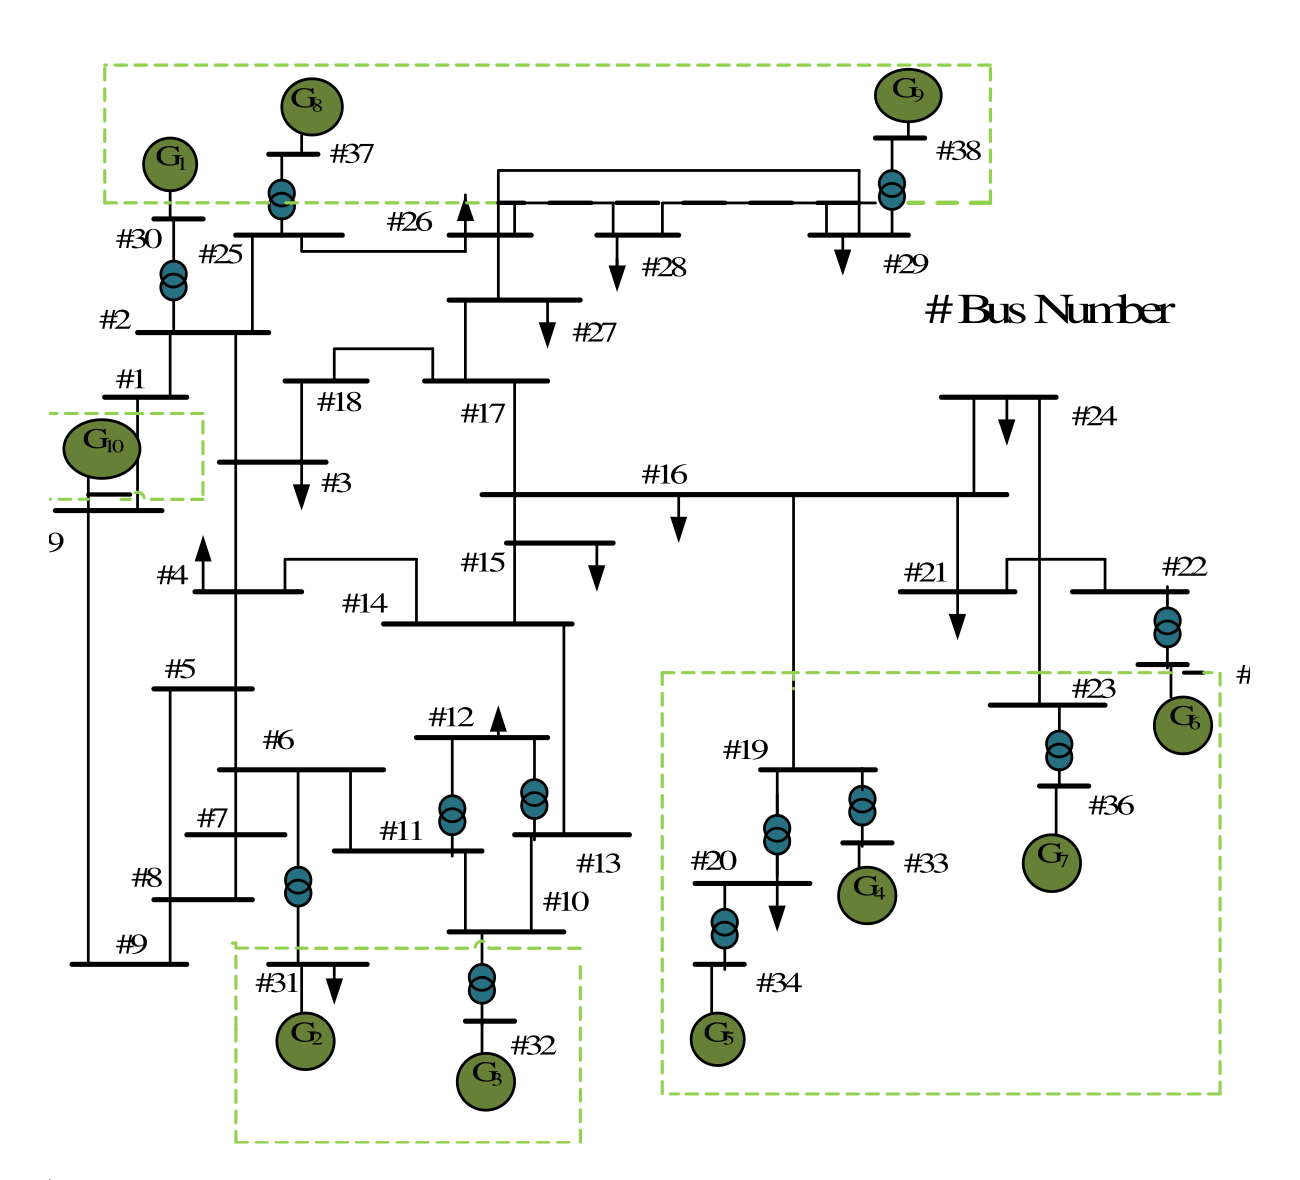
\includegraphics[width=0.72\textwidth]{images/system_figures/ieee39_from_sarkar2024drga.png}
    \caption{Μονογραμμικό διάγραμμα του \textenglish{\textit{IEEE 39-Bus System}}. Πηγή:~\cite{sarkar2024drga}.}
    \label{fig:examined-ieee39-system}
\end{figure}
\FloatBarrier
